\newpage
\section{TGGs in action}
\genHeader
\label{sect:TGGs_in_Action}

In order to perform a forwards or backwards transformation, we need to actually create something for the TGG to work with. In other words, we need to create an
instance model\footnote{For a detailed review of instances and how to create them, refer to Part II, Section 3} of either our target or our source metamodel!
Since dictionaries are a much simpler structure, let's start with the backwards transformation, from \texttt{DictionaryToBox}.

\begin{itemize}

\item[$\blacktriangleright$] Navigate to \texttt{Dictionary\-Language/model/} and open \texttt{Dictio\-nary\-Lang\-uage.ecore}. Create a new
dynamic instance of a \texttt{Dictionary} named \texttt{target.xmi}. Don't quickly close the window by pressing \texttt{finish}! Make sure you persist the
instance in \texttt{Learn\-ing\-Box\-To\-Dictionary\-In\-te\-gra\-tion/in\-stan\-ces/} (Fig.~\ref{fig:create_instance_dict}).

\begin{figure}[htbp]
\begin{center}
  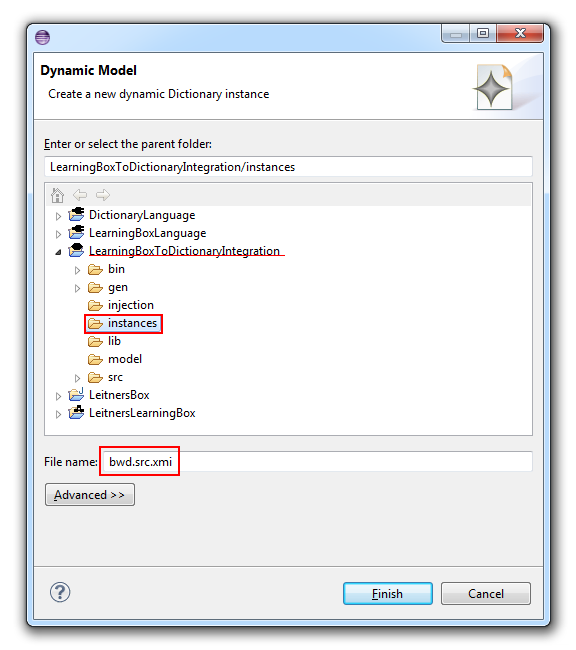
\includegraphics[width=0.8\textwidth]{eclipse_dictionaryInstance}
  \caption{Create a dynamic instance of \texttt{Dictionary}}
  \label{fig:create_instance_dict}
\end{center}
\end{figure}

\newpage

\item[$\blacktriangleright$] Open the new file and edit the \texttt{Dictionary} properties by double-clicking and setting \texttt{Title} to \texttt{English
Numbers} in the \texttt{Properties} tab below the window.

\vspace{0.5cm}

\item[$\blacktriangleright$] Create three child \texttt{Entry} objects, giving each one a different difficulty level. Don't forget the syntax we created for
each \texttt{entry.content} in the \texttt{CardToEntryRule} when setting up the constraints! Be sure to set this property as \texttt{<word>:<meaning>}. Your
\texttt{target.xmi} should quickly resemble Fig.~\ref{fig:dictionaryxmi}.

\vspace{0.5cm}

\begin{figure}[htbp]
\begin{center}
  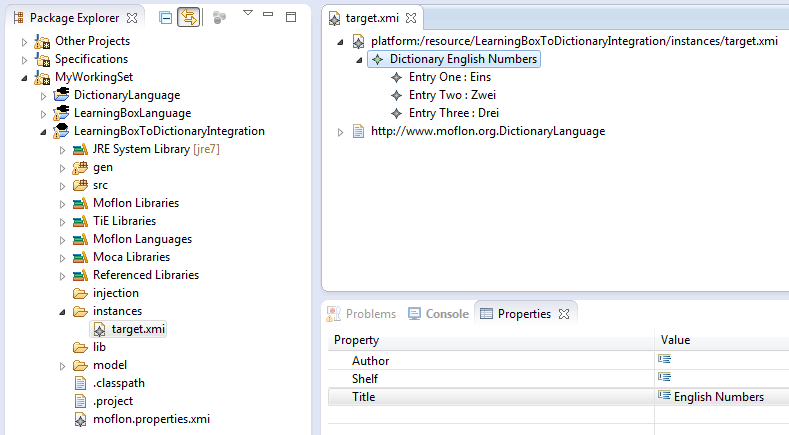
\includegraphics[width=\textwidth]{eclipse_targetThreeEntries}
  \caption{Contents of the dictionary}
  \label{fig:dictionaryxmi}
\end{center}
\end{figure}

\item[$\blacktriangleright$] Navigate to ``LearningBox\-To\-Dictionary\-In\-te\-gra\-tion\-/src'' and right-click on \texttt{TGGMain.java}. Go to ``Run
as\ldots/Java Application''

\vspace{0.5cm}

\item[$\blacktriangleright$] Did you get one error message, followed by one success message in eMoflon console window below the editor?
(Fig.~\ref{fig:tggERROR}) Perfect! Both of these statements make sense -- our TGG first attempted a forward transformation of \texttt{box} to
\texttt{dictionary} but, given that it was missing the source (\texttt{box}) instance, it was only able to perform a transformation in the backwards direction.

\begin{figure}[htbp]
\begin{center}
  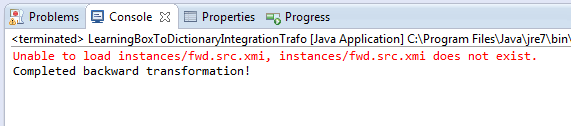
\includegraphics[width=\textwidth]{eclipse_TGGError}
  \caption{comment}
  \label{fig:tggERROR}
\end{center}
\end{figure}

\newpage

\item[$\blacktriangleright$] Refresh the integration's \texttt{instances} folder. There should now be four new \texttt{.xmi} files. While you created
\texttt{target}, the TGG generated \texttt{corr\_BWD}, the correspondence graph between target and source, \texttt{protocol\_BWD}, a listing of the attempted
steps taken (as well as their results), and \texttt{target.xmi\_BWD}, the output of the transformation. Open this file in the editor.

\item[$\blacktriangleright$] Its a \texttt{Box} of \texttt{English Numbers}! Expand the tree and you'll see our \texttt{Dictionary} in its equivalent
\texttt{Box} format containing three \texttt{Par\-ti\-tions} (Fig.~\ref{fig:derivedBOX}). Double click each \texttt{card} and observe how each
\texttt{entry.content} was split into two sides.

\vspace{0.5cm}

\begin{figure}[htbp]
\begin{center}
  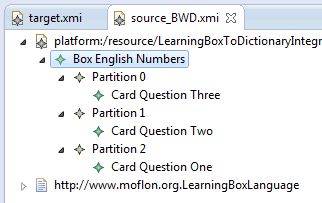
\includegraphics[width=\textwidth]{eclipse_derivedSource}
  \caption{our created box}
  \label{fig:derivedBOX}
\end{center}
\end{figure}

\item[$\blacktriangleright$] Don't forget about one of eMoflon coolest model visualizing features -- the graph viewer! This is an especially useful tool with
TGGs when you need to do a quick confirmation that your transformation was successful. To practice, drag-and-drop \texttt{Box English Numbers} into the
window.\footnote{If the feature window has been closed and is not active on your screen, right-click on the eMoflon perspective and press ``reset''} You can see
the \texttt{partition}s properly connected via link variables, and you can see each \texttt{card} in its proper place (Fig.~\ref{fig:graphViewBox}). 

\begin{figure}[htb]
\begin{center}
  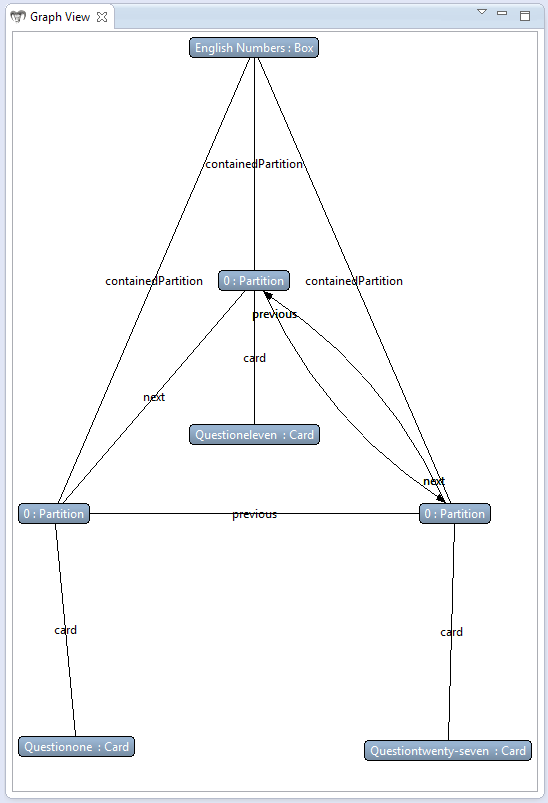
\includegraphics[width=0.6\textwidth]{eclipse_EngNumBoxGraphView}
  \caption{dat graph view. hmmmm.}
  \label{fig:graphViewBox}
\end{center}
\end{figure}

Congratulations! You have successfully performed your first \emph{backward} transformation from your target model (dictionary) to your source (Learning box)
using TGGs! To show that the transformation is actually bidirectional however, let's edit the source model (thus resolving the error), and run the TGG again to
transform a \texttt{Box} forward into a \texttt{Dictionary}.


\item[$\blacktriangleright$] Make a copy of \texttt{target.xmi\_BWD.xmi} (the result of the backward transformation)
and rename it to \texttt{source.xmi}.
  
% \item[$\blacktriangleright$] Open \texttt{source.xmi} and create some new \texttt{Card} objects in the \texttt{Partition}s (e.g., create a new \texttt{Card}
% with \texttt{Card.face = ``Question : two''}, \texttt{Card.back = ``Answer : zwei''} in \texttt{Partition 0}).

\item[$\blacktriangleright$] Run the \texttt{TGGMain.java} again by pressing the green ``Run As\ldots'' icon on the toolbar. You should now have two success
messages in the console window! Refresh the ``instances" folder and compare \texttt{source.xmi\_FWD.xmi} against the original target model. If everything was
created and executed properly, they should look exactly the same. Great job!

\end{itemize}
